% Notes on the Rouy and Tourin Shape from Shading Model

\documentclass[11pt]{article}

\usepackage{amsmath}
\usepackage{amsfonts}
\usepackage{graphicx,color,geometry}
\usepackage{subcaption}
\usepackage{hyperref}

\newtheorem{definition}{Definition}
\newtheorem{example}{Example}

\begin{document}
	\title{\textbf{Notes on SfS - Orthographic Projection Model by Rouy and Tourin }}
	\author{\textit{Balaje K \& Sanath Keshav}}
	\date{\today}
	\maketitle
	
	\section{Viscosity Solutions}
	The classic orthographic Shape from Shading (SfS) model was developed by Rouy and Tourin, who presented the viscosity solution approach to solving the SfS Problem. The Model is described by a non-linear first order PDE, known as the Eikonal Equation (A Hamilton Jacobi Equation).
	\begin{equation}
		|\nabla u| = n(x)
	\end{equation}
	where $n(x)$ is the source term. No solution exists in $C^1$, the proof of which is shown below.\\
	
	\noindent
	\begin{example}
		Consider the following Boundary Value Problem
		\begin{eqnarray}\label{eq:1}
		|\nabla u| &=& 1 \;\;\;\; \text{in} \;\; \Omega = (0,1) \\
		u &=& 0 \;\;\;\; \text{on} \;\; \partial \Omega = \{0,1\}\label{eq:2}
		\end{eqnarray}
		Suppose if some $u \in C^1$, and as $u(0)=u(1)=0$, by Rolle's Theorem $\exists\;\; x_0 \in (0,1)$ such that $u'(x_0) = 0$. This exactly contradicts (\ref{eq:1}), that $|u'| = 1$ on the entire domain. So $u \notin C^1$. \\
	\end{example}
	
	\noindent
	This is exactly why we are required to find the solutions which are in some sense, ``weak" solutions to the problem \cite{yong}. For example, $u^+(x) = \frac{1}{2}- \left|\frac{1}{2} - x\right|$ is a solution to the problem discussed above. We see that $u \in C^0$ but $u \notin C^1$. But on the other hand, we see that this is not the only solution i.e., $u^-(x) = \left | \frac{1}{2} - x\right | - \frac{1}{2}$ is also a solution to the problem. So, the question of uniqueness arises.\\
	
	\noindent
	We are now in need of a theory which addresses the issue of existence and uniqueness. P.L.Lions and M.Crandall, came up with a theory known as \textbf{viscosity solutions} \cite{lions} that describes a way to obtain a unique solution to the class of PDEs known as \textbf{Hamilton Jacobi Equations}. This concept was obtained from the vanishing viscosity method, which involves adding an artificial viscosity term $\epsilon u_{xx}$ to the PDE and letting $\epsilon \to 0$. With this Crandall and Lions were able to conclude that for problem (\ref{eq:1}) - (\ref{eq:2}), the unique solution is in fact
	\begin{equation}
		u(x) = u^+(x) = \frac{1}{2}- \left|\frac{1}{2} - x\right| .
	\end{equation}
	To see why this is the case we define the following.
	\begin{definition}Viscosity Sub- and Super- solution\\
		
		Consider the following Hamilton-Jacobi Equation
		\begin{equation}
			H(x, \nabla u) = 0.
		\end{equation}
		\begin{enumerate}
			\item
			$u \in C^0$ is a viscosity sub-solution of the HJE; if for any $\phi \in C^1$, if $u-\phi$ attains the maximum at $x_0$, then
			\begin{equation}
			H(x_0,\nabla \phi) \le 0
			\end{equation}
			
			\item
			$u \in C^0$ is a viscosity super-solution of the HJE; if for any $\phi \in C^1$, if $u-\phi$ attains the minimum at $x_1$, then
			\begin{equation}
			H(x_1,\nabla \phi) \ge 0
			\end{equation}
		\end{enumerate}
		
		Any $u \in C^0$ is a viscosity solution if $u$ is both a viscosity sub- and super- solution.
	\end{definition}
	
	\noindent
	Now consider the Eikonal equation in 1D,
	\begin{eqnarray}
		|u'(x)| &=& 1 \;\;\;\; x \in (-1,1)\\
		u &=& 0 \;\;\;\; x \in \{-1,1\}
	\end{eqnarray}
	The Hamiltoinan $H(x,p) = |p|-1$ where $p = \nabla u$, is a convex function in $p$. We now show that the solution $u^+(x) = 1-|x|$ is the viscosity solution to the problem.\\
	
	\noindent
	\textbf{Proof:} Let $u - \phi$ attain maximum at $x_0$. In this case $x_0 = 0$. \\
	
	\noindent
	This means,
	\begin{eqnarray}
			u(x_0) - \phi(x_0) &\ge& u(x) - \phi(x) \;\;\;\; \forall x \in (-1,1)\\
			\implies \phi(x) - \phi(x_0) &\ge& u(x) - u(x_0) \label{eq:3}
	\end{eqnarray}
	
	\noindent
	If $x>x_0 = 0$, we have from (\ref{eq:3})
	\begin{eqnarray}
		\frac{\phi(x) - \phi(x_0)}{x-x_0} &\ge& \frac{u(x) - u(x_0)}{x-x_0}		\\
		\implies \lim\limits_{x\to x_0} \frac{\phi(x) - \phi(x_0)}{x-x_0} &\ge& \lim\limits_{x\to x_0} \frac{u(x) - u(x_0)}{x-x_0} \\
		\implies \lim\limits_{x\to x_0} \frac{\phi(x) - \phi(x_0)}{x-x_0} &\ge& \lim\limits_{x\to x_0} \frac{1-x - (1)}{x}\\\nonumber\\
		\phi'(x) &\ge& -1 \label{eq:4}		
	\end{eqnarray}
	If $x < x_0 = 0$, we follow the same procedure to get, 
	\begin{equation}
		\phi'(x) \le 1	\label{eq:5}
	\end{equation}
	Thus from (\ref{eq:4}) \& (\ref{eq:5}), we get $|\phi'(x)| \le 1$, which shows that $u^+$ is a sub-solution to the Eikonal Equation. One can verify that $u^+$ satisfies the super-solution condition as well and thus is a viscosity solution to the problem, which completes the proof.\\
	
	\noindent
	It is easy to see that, by using the same steps ,that $u^-(x) = |x| - 1$ is \textbf{not a viscosity solution} if we choose the Hamiltonian $H(x,p) = |p|-1$, but \textbf{is indeed a viscosity solution} for the Hamiltonian $H(x,p) = 1 - |p|$. Thus the viscosity solution is dependent on the nature of the Hamiltonian we choose, i.e., (concave / convex).\\
	
	\noindent
	Let us consider the special case where the Eikonal Equation is,
	\begin{equation}
		|\nabla u | = 0
	\end{equation}
	This particular PDE presents us with a huge problem of \textbf{uniqueness}. This is evident from the sub-solution definition, that 
	\begin{eqnarray}
		H(x,\nabla \phi) \le 0\\
		\implies |\nabla \phi| \le 0
	\end{eqnarray} 
	which cannot be satisfied for all cases, as $|\nabla \phi| \ge 0$. This particular case is a problem when we consider the numerical solution of the Shape from Shading Model proposed by Rouy and Tourin.

	
	\section{Shape from Shading}
	The model propsed by Rouy and Tourin\cite{rouy} for an orthographic shape from shading model, with the light source vertically above the object, is given by
	\begin{equation}
		|\nabla u(x)| = \sqrt{\frac{1}{I(x)^2} - 1}, \;\;\;\; x \in \Omega \subset \mathbb{R}^2
	\end{equation}
	Rouy and Tourin proposed to solve the PDE by modelling it as a transient problem and then solving till the steady state is reached, i.e.,
	\begin{equation}
		u_t + |\nabla u| = \sqrt{\frac{1}{I^2} - 1}
	\end{equation}
	
	\noindent
	Sethian\cite{sethian} proposed a variant of the Einguist Osher scheme to solve the Eikonal Equation. Instead, one can use any upwind scheme (like Godunov for ex.) to solve the transient equation.\\
	
	\noindent
	Now, if $0 < I(x) < 1$, we solve the PDE by normally applying the boundary conditions and the scheme converges to the unique viscosity solution. In some cases, if $ I(x) = 1$ locally, we have a problem of uniqueness, which was discussed above. Presenting an illustration with,
	\begin{equation}
		I(x,y) = \frac{1}{\sqrt{1+ (16y(1-y)(1-2x))^2 + (16x(1-x)(1-2y))^2}}
	\end{equation}
	It is easy to see that \textbf{one of the solution} (the other possible one is obviously the negative of this curve) is given by $u(x,y) = 16x(1-x)y(1-y)$. This exact solution is shown in the Figure \ref{fig:1},
	\begin{figure}[h!]
		\centering
		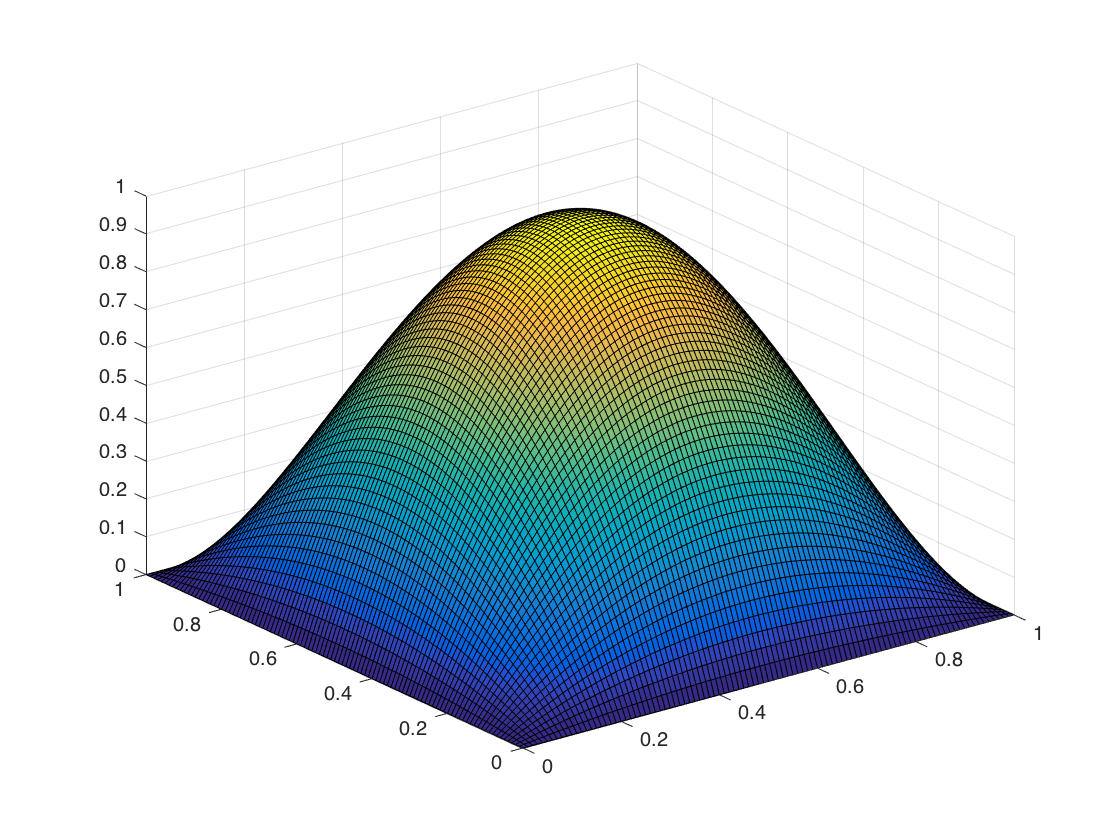
\includegraphics[scale = 0.3]{exact.png}
		\caption{Exact Solution}
		\label{fig:1}
	\end{figure}
	
	\noindent
	Now, $I(x=0.5,y=0.5) = 1$ and $u(x=0.5,y=0.5) = 1$. Not accounting for the value of $u(x,y)$ at places where $I(x,y) = 1$, can produce devastating effects as shown in Figure \ref{fig:2}. The data prescribed by the initial data is just inaccurately carried over by the scheme, if not handled properly.
	\begin{figure}[h!]
		\begin{subfigure}{0.5\textwidth}
			\centering
			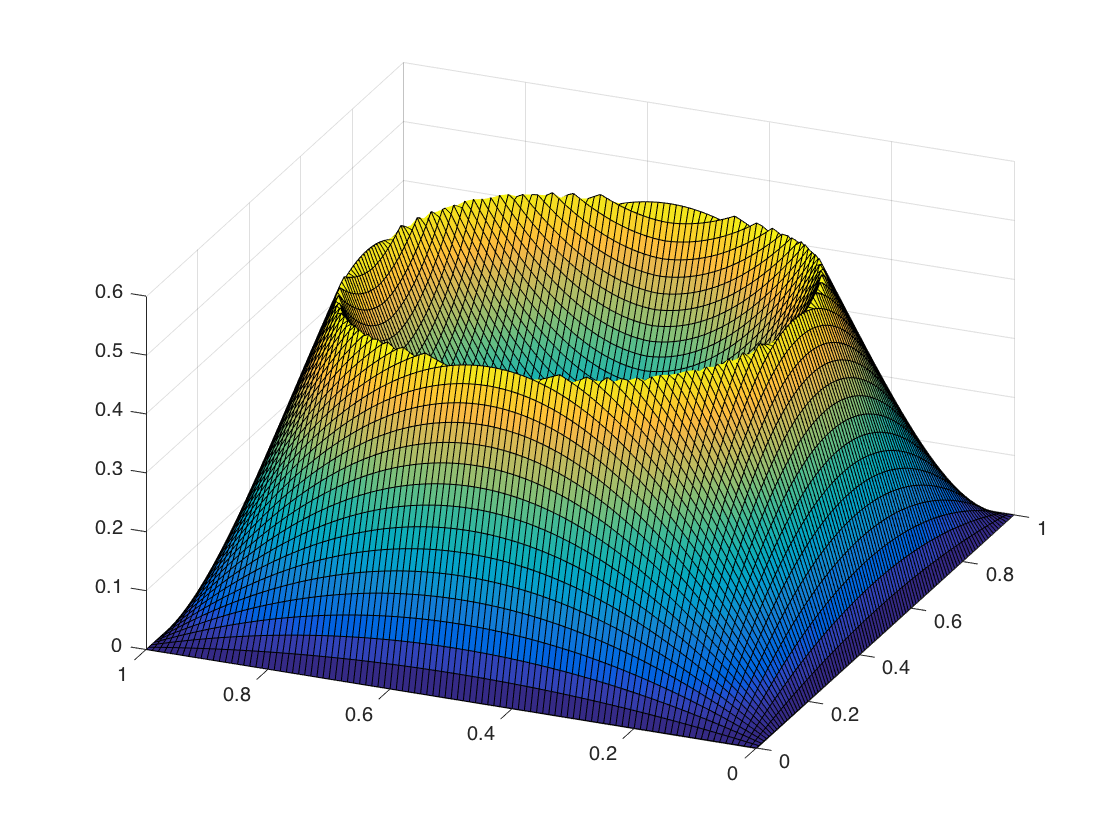
\includegraphics[width = 8cm, height = 7cm]{wrong.png}
			\subcaption{Wrong Result}
			\label{fig:2}
		\end{subfigure}
		\begin{subfigure}{0.5\textwidth}
			\centering
			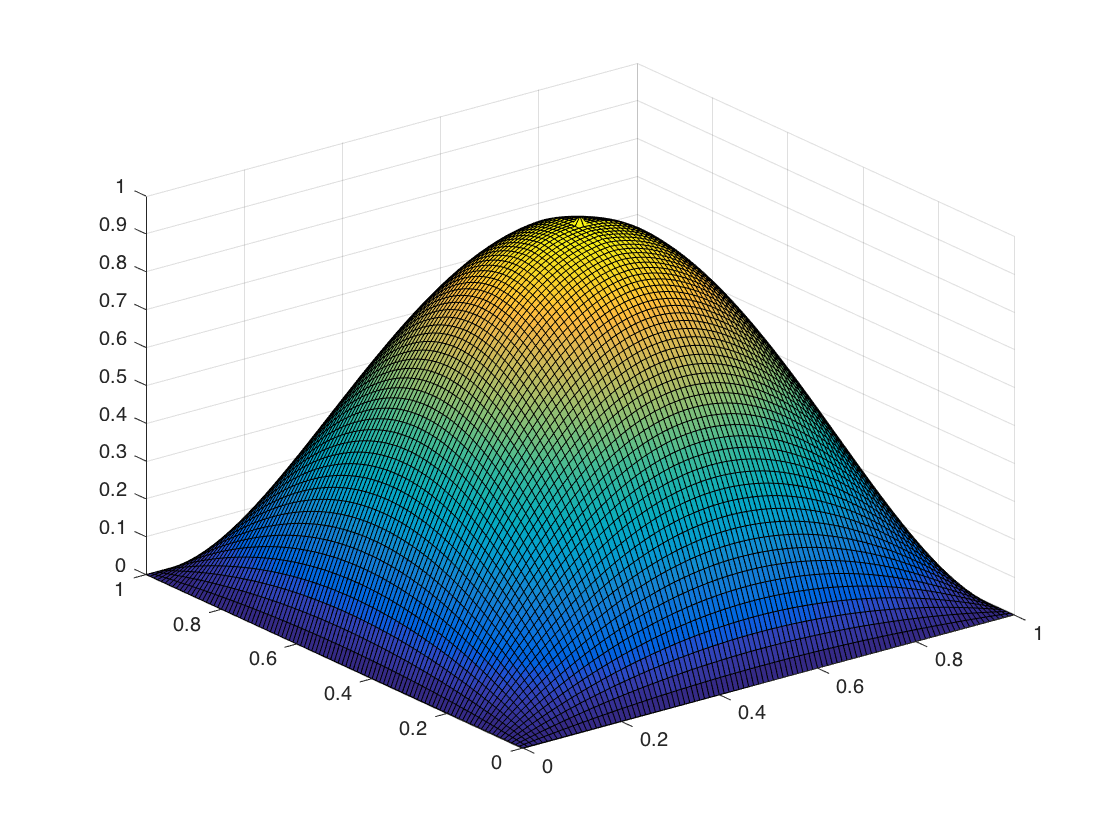
\includegraphics[width = 8cm, height = 7cm]{correct.png}
			\caption{Physically Relevant Result}
			\label{fig:3}
		\end{subfigure}
	\end{figure}
	The correct result can be obtained by \textbf{manually setting} the value of $u(x,y)$ at places where $I(x_i,y_j) = I_{ij} = 1$. This is done by constructing an Index Set $Q$ where,
	\begin{equation}
		Q_{ij} = \begin{Bmatrix}
		1 & I_{ij} \ne 1\\
		0 & I_{ij} = 1
		\end{Bmatrix}		
	\end{equation}
	
	\noindent
\textbf{So to get the physically relevant solution, we set $u_{ij} = 1$ where $Q_{ij} = 0$.} Shown in Figure \ref{fig:3}.\\
	
	\noindent
	Prados and Faugeras\cite{prados}, came up with a Generic Hamiltonian that combines both Orthographic and Perspective Projection Models. The Hamiltonian that they came up with, satisfies convexity, coercivity and regularity.  Subsolution condition is satisfied as long as $0<I(x)<1$, and the uniqueness is lost as soon as $I(x) = 1$. This is a major challenge is that we are unable to correctly reconstruct the image, if we do not know what happens at places where $I(x) = 1$ - called the \textbf{singularity points}.
	
	\section{Results}
	An attempt to reconstruct the follwing classical \textbf{text vase} from the intensity image shown in Figure \ref{fig:4}, was made using the Orthographic projection model. The result is shown in Figure \ref{fig:5}. Homogeneous Neumann boundary conditions are employed on the boundaries.
		\pagebreak
	\begin{figure}[h!]
		\centering
		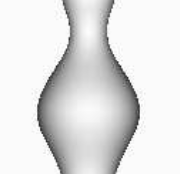
\includegraphics[scale = 1.5]{vase.png}
		\caption{Test Vase}
		\label{fig:4}
	\end{figure}
	\begin{figure}[h!]
		\centering
			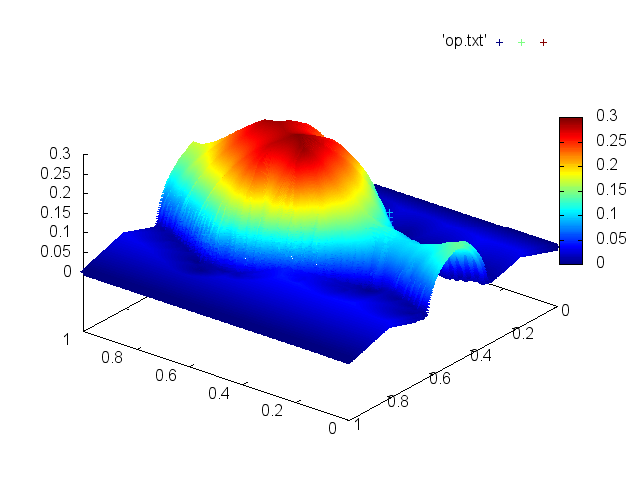
\includegraphics[scale = 0.8]{vase_gnuplot.png}
			\caption{Reconstruction using Orthographic Projection}
			\label{fig:5}
	\end{figure}
		\pagebreak
	\nocite{*}
	\bibliographystyle{acm}
	\bibliography{biblio}
\end{document}
